\documentclass[11pt,a4paper]{article}
\usepackage[utf8]{inputenc}
\usepackage{amsmath,amsfonts,amssymb}
\usepackage{graphicx}
\usepackage{geometry}
\geometry{margin=1in}
\usepackage{booktabs}
\usepackage{hyperref}
\usepackage{float}
\usepackage{xcolor}

\definecolor{darkbg}{HTML}{0d121f}
\definecolor{lighttext}{HTML}{e2e8f0}
\definecolor{primary}{HTML}{8b5cf6}
\definecolor{secondary}{HTML}{0dd5c5}

\pagecolor{darkbg}
\color{lighttext}

\hypersetup{
    colorlinks=true,
    linkcolor=secondary,
    urlcolor=secondary
}

\title{\textbf{EE3621: Digital Signal Processing} \\ \Large Lecture 19: Digital Filter Structures — FIR Structures \& Lattice Filters \\ \large (III B.Tech EEE)}
\author{Lecture Notes (40-Minute Plan)}
\date{}

\begin{document}

\maketitle

\section{Lecture Plan \& Objectives (40 Minutes Breakdown)}
\begin{itemize}
    \item \textbf{00:00 -- 05:00 (5 mins):} Introduction to FIR Transversal Structures and Direct Convolution.
    \item \textbf{05:00 -- 10:00 (5 mins):} Linear Phase FIR Exploitation and complexity reduction.
    \item \textbf{10:00 -- 17:00 (7 mins):} FIR Lattice Structure, PARCOR coefficients, forward/backward prediction.
    \item \textbf{17:00 -- 22:00 (5 mins):} Levinson-Durbin algorithm mapping direct form to lattice.
    \item \textbf{22:00 -- 26:00 (4 mins):} IIR Lattice-Ladder structures for pole-zero models.
    \item \textbf{26:00 -- 30:00 (4 mins):} Polyphase FIR Decomposition for decimation/interpolation.
    \item \textbf{30:00 -- 35:00 (5 mins):} Fast Convolution: Overlap-Save and Overlap-Add.
    \item \textbf{35:00 -- 37:00 (2 mins):} Hardware Implementation (MAC units, pipelining).
    \item \textbf{37:00 -- 40:00 (3 mins):} Checkpoints and Q\&A.
\end{itemize}

\noindent\rule{\textwidth}{0.5pt}

\section{FIR Transversal (Tapped-Delay-Line) Structure}
An FIR filter of length $M$ (order $N = M-1$) performs a direct convolution sum:
\begin{equation}
y[n] = \sum_{k=0}^{M-1} h[k]x[n-k]
\end{equation}

\textbf{Step-by-Step Expansion:}
\begin{enumerate}
    \item At time $n$, the output is:
    \begin{equation}
    y[n] = h[0]x[n] + h[1]x[n-1] + \dots + h[M-1]x[n-M+1]
    \end{equation}
    \item This implies we need current and past input samples: $x[n], x[n-1], \dots, x[n-M+1]$.
    \item To store these, we require $M-1$ delay elements ($z^{-1}$ blocks).
    \item Each delayed sample is multiplied by a tap weight $h[k]$. This gives $M$ multipliers.
    \item The products are summed together using $M-1$ adders.
\end{enumerate}

\textbf{Engineering Intuition:} This is called a \textbf{tapped-delay-line} because the signal propagates down a chain of delay registers, and at each stage we ``tap'' the line, multiply by a coefficient, and accumulate. Since there is no feedback loop, the system is unconditionally stable.

\textbf{Computational Complexity:} For every output sample $y[n]$, we compute exactly $M$ multiplications and $M-1$ additions. In real-time DSP, $M$ MAC (Multiply-Accumulate) operations per sample determine the required processing bandwidth.

\section{Exploiting Linear Phase in FIR Filters}
If an FIR filter has a symmetric (or anti-symmetric) impulse response, it has exact linear phase. For a symmetric filter:
\begin{equation}
h[n] = h[M-1-n]
\end{equation}

\textbf{Complexity Reduction Derivation:}
\begin{enumerate}
    \item Let's assume $M$ is odd. The center tap is at $(M-1)/2$.
    \item The convolution sum is:
    \begin{equation}
    y[n] = \sum_{k=0}^{M-1} h[k]x[n-k]
    \end{equation}
    \item Split the sum into two halves and the center tap:
    \begin{equation}
    y[n] = \sum_{k=0}^{(M-3)/2} h[k]x[n-k] + h[(M-1)/2]x[n-(M-1)/2] + \sum_{k=(M+1)/2}^{M-1} h[k]x[n-k]
    \end{equation}
    \item In the second sum, let $m = M - 1 - k$. Then $k = M - 1 - m$.
    \item The sum bounds become $m = 0$ to $(M-3)/2$.
    \begin{equation}
    \sum_{m=0}^{(M-3)/2} h[M-1-m]x[n-M+1+m]
    \end{equation}
    \item Using the symmetry property $h[M-1-m] = h[m]$:
    \begin{equation}
    \sum_{m=0}^{(M-3)/2} h[m]x[n-M+1+m]
    \end{equation}
    \item Recombine the sums by factoring out $h[k]$:
    \begin{equation}
    y[n] = \sum_{k=0}^{(M-3)/2} h[k] \left( x[n-k] + x[n-M+1+k] \right) + h[(M-1)/2]x[n-(M-1)/2]
    \end{equation}
\end{enumerate}

\textbf{KEY RESULT:} Instead of $M$ multiplications, we only need $(M+1)/2$ multiplications. The adders increase slightly because we add the symmetric delayed samples before multiplication, but multipliers are much more expensive in hardware than adders. Halving the number of multipliers saves significant silicon area.

\section{FIR Lattice Structure}
Lattice structures offer a highly modular, stage-by-stage way to implement filters. They are widely used in speech processing (Linear Predictive Coding) and adaptive filters.

\subsection{All-Zero Lattice}
The lattice structure connects forward prediction errors $f_m[n]$ and backward prediction errors $b_m[n]$ at stage $m$. The parameters defining the lattice are the \textbf{PARCOR} (Partial Correlation) coefficients or reflection coefficients, $K_m$.

\textbf{The Recursion Equations:} For $m = 1, 2, \dots, M-1$, we have:
\begin{enumerate}
    \item $f_0[n] = b_0[n] = x[n]$
    \item Forward error update:
    \begin{equation}
    f_m[n] = f_{m-1}[n] + K_m b_{m-1}[n-1]
    \end{equation}
    \item Backward error update:
    \begin{equation}
    b_m[n] = K_m^* f_{m-1}[n] + b_{m-1}[n-1]
    \end{equation}
\end{enumerate}

\textbf{Engineering Intuition:}
\begin{itemize}
    \item $f_m[n]$ represents the error in predicting $x[n]$ from $m$ past samples.
    \item $b_m[n]$ represents the error in predicting $x[n-m]$ from $m$ future samples.
    \item As we add stages, we are orthogonalizing the signal.
    \item \textbf{Advantage:} If we want to increase the filter order, we simply tack on another lattice stage without recalculating the previous $K_m$ coefficients (unlike direct form, where increasing order changes all coefficients).
\end{itemize}

\section{Relationship Between FIR Coefficients and PARCOR}
How do we find $K_m$ given $h[n]$ (where $h[0]=1$ for a monic polynomial)?
The \textbf{Levinson-Durbin algorithm} recursively bridges the direct form coefficients $\alpha_m(k)$ and lattice coefficients $K_m$.

\textbf{Derivation (Step-down recursion):} Given the $m$-th order polynomial $A_m(z) = 1 + \sum_{k=1}^m \alpha_m(k) z^{-k}$.
\begin{enumerate}
    \item The reflection coefficient is the highest order coefficient:
    \begin{equation}
    K_m = \alpha_m(m)
    \end{equation}
    \item Compute the $(m-1)$-th order coefficients:
    \begin{equation}
    \alpha_{m-1}(k) = \frac{\alpha_m(k) - K_m \alpha_m(m-k)}{1 - K_m^2} \quad \text{for } k = 1, 2, \dots, m-1
    \end{equation}
    \item Repeat this step down to $m=1$.
    \item The system is minimum phase (all zeros inside the unit circle) if and only if $|K_m| < 1$ for all $m$.
\end{enumerate}

\section{IIR Lattice-Ladder Structure}
While FIR filters use an all-zero lattice, IIR filters require feedback, forming an all-pole (AR) lattice. 
For a general pole-zero IIR system (ARMA), we use a combined \textbf{Lattice-Ladder} structure.

\subsection{All-Pole Lattice (Feedback)}
Instead of predicting forward, we run the lattice backward to synthesize the signal:
\begin{enumerate}
    \item $f_{m-1}[n] = f_m[n] - K_m b_{m-1}[n-1]$
    \item $b_m[n] = K_m f_{m-1}[n] + b_{m-1}[n-1]$
\end{enumerate}
This forms the denominator $1/A(z)$.

\subsection{Ladder Section (Feedforward zeros)}
To implement zeros $B(z)$, we tap the backward error signals $b_m[n]$ (which form an orthogonal basis) and sum them using ladder coefficients $v_m$:
\begin{equation}
y[n] = \sum_{m=0}^M v_m b_m[n]
\end{equation}

\textbf{Comparison to Parallel Form:}
In a previous lecture, we looked at the Parallel IIR structure, which breaks $H(z)$ into parallel sum of Second Order Sections. For context, recall the Parallel IIR structure:
\begin{figure}[H]
\centering
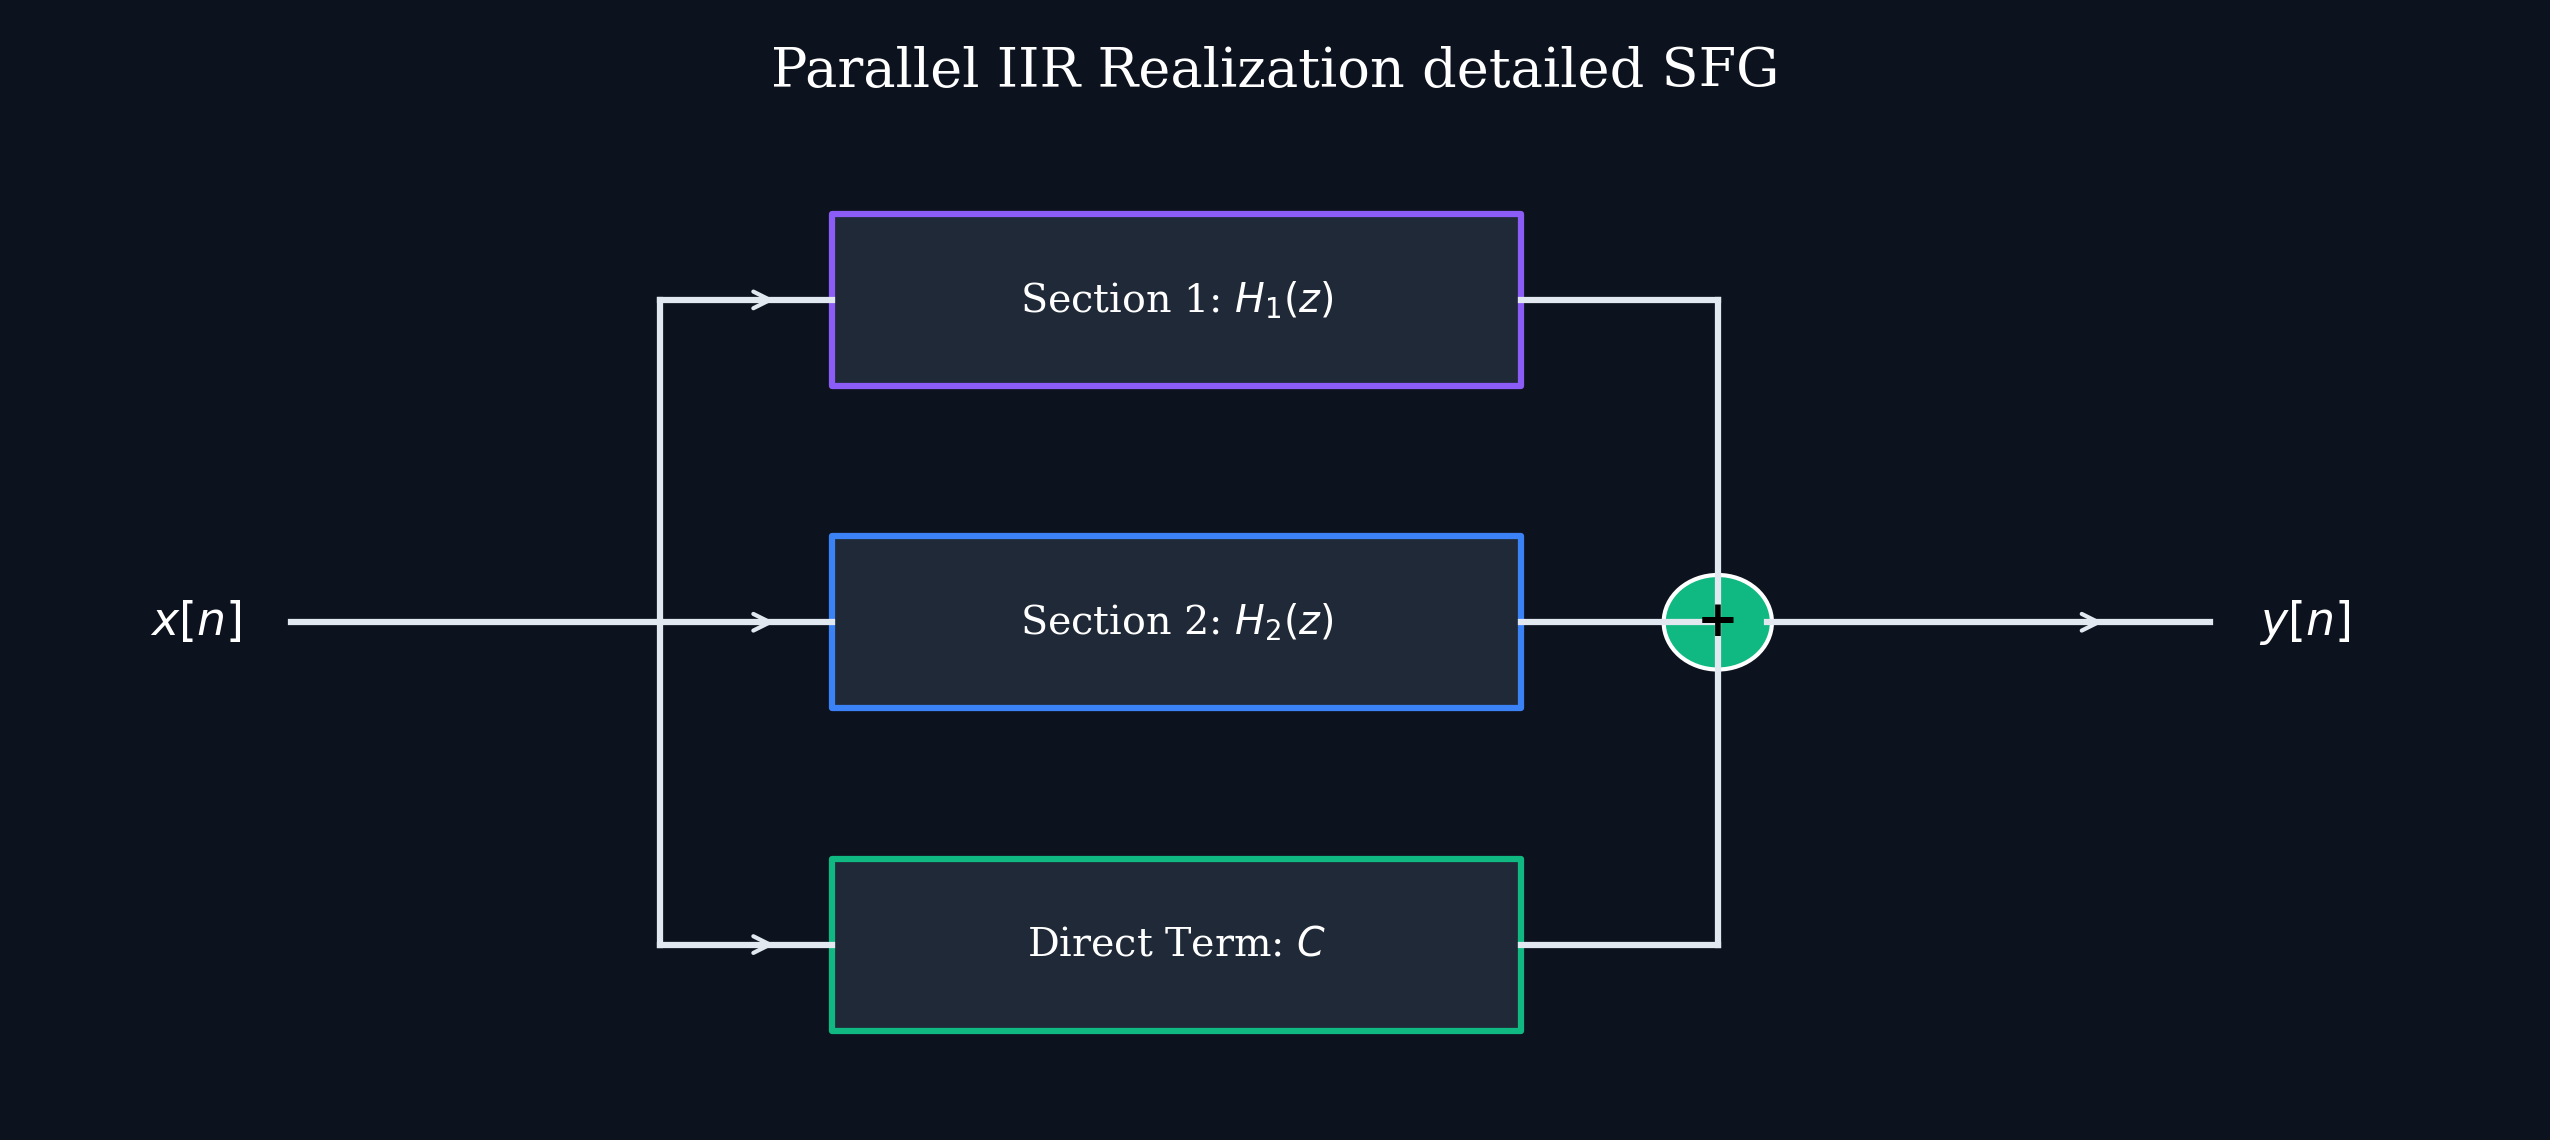
\includegraphics[width=0.7\textwidth]{images/iir_parallel_sfg.png}
\caption{Parallel IIR Signal Flow Graph.}
\label{fig:iir_parallel_sfg}
\end{figure}
While the parallel form prevents coefficient quantization errors from affecting other poles, the Lattice-Ladder form gives robust stability checking ($|K_m| < 1$) even under severe quantization.

\section{Polyphase FIR Decomposition}
When dealing with multirate DSP (decimation or interpolation), computing the full convolution before downsampling wastes power.
Let $M$ be the decimation factor. We decompose $H(z)$ into $M$ polyphase components $E_k(z)$:
\begin{enumerate}
    \item The transfer function is: $H(z) = \sum_{n=0}^{N-1} h[n]z^{-n}$
    \item Group the terms by index modulo $M$:
    \begin{equation}
    H(z) = \sum_{k=0}^{M-1} z^{-k} \left( \sum_{n=0}^{\infty} h[nM+k] (z^M)^{-n} \right)
    \end{equation}
    \item Define the $k$-th polyphase component: $E_k(z) = \sum_{n=0}^{\infty} h[nM+k] z^{-n}$
    \item The filter is exactly represented as:
    \begin{equation}
    H(z) = \sum_{k=0}^{M-1} z^{-k} E_k(z^M)
    \end{equation}
\end{enumerate}
By pushing the downsampler through the filter, we compute the convolution at the lower sample rate, reducing computational workload by a factor of $M$.

\section{Block Processing: Overlap-Save and Overlap-Add}
For very long FIR filters, time-domain convolution $O(N^2)$ is too slow. We use the FFT for fast convolution, which is $O(N \log N)$.
\begin{itemize}
    \item \textbf{Overlap-Add Method:} Break input into non-overlapping blocks of length $L$. Pad and FFT. Output block length is $L+M-1$. Add the tail of size $M-1$ to the start of the next block.
    \item \textbf{Overlap-Save Method:} Break input into overlapping blocks of length $N_{fft}$. The first $M-1$ samples are saved from the previous block. Compute circular convolution. Discard the first $M-1$ samples (time-aliasing), keep the rest.
\end{itemize}

\section{Hardware Implementation Considerations}
When designing an FIR filter on an ASIC or FPGA:
\begin{itemize}
    \item \textbf{MAC Units:} DSP slices in FPGAs are specifically optimized for $A \times B + C$.
    \item \textbf{Pipelining:} Adding pipeline registers between multiplier and adder adds latency but drastically improves maximum clock frequency $f_{max}$.
    \item \textbf{Area vs. Speed:} Fully parallel uses $M$ multipliers and outputs one sample per clock. Fully serial uses 1 multiplier and computes 1 tap per cycle.
\end{itemize}

\section{Checkpoint Questions}
\textbf{Q1:} Given an FIR filter with $h[n] = \{1, 2.5, 2.5, 1\}$, determine the number of multipliers required if linear phase symmetry is exploited.
\newline \textbf{Answer:} Length $M = 4$. Symmetric coefficients: $h[0]=h[3]=1$, $h[1]=h[2]=2.5$. Using symmetry, $y[n] = 1(x[n] + x[n-3]) + 2.5(x[n-1] + x[n-2])$. Need $M/2 = 2$ multipliers.

\vspace{0.5cm}
\textbf{Q2:} A 100-tap FIR filter processes a 10 kHz audio signal. Compare MACs/sec for direct convolution vs. decimation-by-4 using polyphase.
\newline \textbf{Answer:} Direct: $M=100$, so $1,000,000$ MACs/sec. Polyphase Decimation ($M=4$): output rate $2.5$ kHz. 4 polyphase filters of length 25. Each output requires 100 MACs, computed at 2.5 kHz. Total MACs/sec = $250,000$. Computation drops by factor of 4.

\vspace{0.5cm}
\textbf{Q3:} In Overlap-Save, why do we discard the first $M-1$ samples?
\newline \textbf{Answer:} FFT computes circular convolution. The transient response takes $M-1$ samples to settle. In circular convolution, these wrap around and cause time-aliasing, corrupting the first $M-1$ samples, which must be discarded.

\section{Key Formulas}
\begin{table}[H]
\centering
\begin{tabular}{@{}ll@{}}
\toprule
Concept & Formula \\ \midrule
FIR Difference Equation & $y[n] = \sum_{k=0}^{M-1} h[k]x[n-k]$ \\
Linear Phase Output (odd M) & $y[n] = \sum_{k=0}^{(M-3)/2} h[k] ( x[n-k] + x[n-M+1+k] ) + h[\frac{M-1}{2}]x[n-\frac{M-1}{2}]$ \\
Lattice Forward Error & $f_m[n] = f_{m-1}[n] + K_m b_{m-1}[n-1]$ \\
Lattice Backward Error & $b_m[n] = K_m^* f_{m-1}[n] + b_{m-1}[n-1]$ \\
Polyphase Decomposition & $H(z) = \sum_{k=0}^{M-1} z^{-k} E_k(z^M)$ \\ \bottomrule
\end{tabular}
\end{table}

\end{document}
